\documentclass{article}
\usepackage{amsmath,tikz,algorithm2e}
\usetikzlibrary{matrix,calc}
\title{Computer\/ Robot Vision: Lecture 3}
\author{Sam Barrett}

\begin{document}
\maketitle

\section{Image Gradients \& Edges}

\subsection{Edge Detection}
\label{subsec:edge detection}

The goal of edge detection is to take an image and map it from a 2D array of pixel values to a set of curves, line segments or contours. In so doing we filter out less relevant information whilst preserving important structural properties.

The main idea is to look for strong gradients in the pixel values. This allows us to loosly define an edge as a \textit{place of rapid change in the image intensity function}. The first derivative of the intensity function over a horizontal section of pillar should show two spikes corresponding to each edge of the object.

We can express the partial derivative $f(x,y)$ for a 2D function as:

\[
  \frac{\delta f(x,y)}{\delta x} = \lim_{\varepsilon \rightarrow 0} \frac{f(x+ \varepsilon, y)- f(x,y)}{\varepsilon}
\]

For discrete data, such as images, we can approximate this using \textit{finite differences}:

\[
  \frac{\delta f(x,y)}{\delta x} = \frac{f(x+1,y)-f(x,y)}{1}
\]

We can also efficiently perform this operation using matrix convolution. We can think of an image gradient as being separate in the $x$ and $y$ direction, as such we must calculate the image gradient of both, $\frac{\delta f(x,y)}{\delta x} $ and $\frac{\delta f(x,y)}{\delta y} $

The filter for constructing the $x$ derivative is simply:


\begin{center}
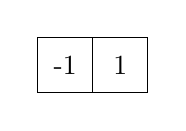
\begin{tikzpicture}
\matrix (m) [matrix of nodes,
             nodes={minimum size=1em, outer sep=0pt,inner sep=0,line
             width=0.5pt,append after command={\pgfextra{\draw
             ($(\tikzlastnode.north west)+(-0.5em,+0.5em)$)
             rectangle ($(\tikzlastnode.south east)+(0.5em,-0.5em)$);}}},
             nodes in empty cells,column sep=-0.5pt, row sep=-0.5pt
              ]
              {
                -1 & 1 \\
  };
\end{tikzpicture}
\end{center}

The filter for the $y$ direction is: \textbf{check}

\begin{center}
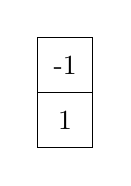
\begin{tikzpicture}
\matrix (m) [matrix of nodes,
             nodes={minimum size=1em, outer sep=0pt,inner sep=0,line
             width=0.5pt,append after command={\pgfextra{\draw
             ($(\tikzlastnode.north west)+(-0.5em,+0.5em)$)
             rectangle ($(\tikzlastnode.south east)+(0.5em,-0.5em)$);}}},
             nodes in empty cells,column sep=-0.5pt, row sep=-0.5pt
              ]
              {
                -1 \\
                1 \\
  };
\end{tikzpicture}
\end{center}

The image gradient can be obtained as the partial derivative of the intensity values of an image in the $x$ and $y$ direction and can be denoted as:

\[
  \nabla f = \left[ \frac{\delta f}{\delta x}, \frac{\delta f}{\delta y}\right]
\]

With this value we can define:

\begin{itemize}
  \item The \textbf{gradient direction}, or orientation of edge normal. It is given by:

        \[
        \theta = \tan^{-1}(\frac{\delta f}{\delta y}/ \frac{\delta f}{\delta x})
        \]

  \item The edge or gradient \textbf{strength} is given by the gradient magnitude:

        \[
        \| \nabla f \| = \sqrt{\left(\frac{\delta f}{\delta x}\right)^{2} + \left(\frac{\delta f}{\delta y}\right)^{2}}
        \]


\end{itemize}

\subsubsection{Effects of noise}

For any real-life image, if we consider a single row or column of the image and plot its intensity as a function we see a noisy signal. This noise effects our derivative as this noise is amplified by derivation.

Different filters have different sensitivity to noise. What can we do to tackle it?

One solution is to \textit{smooth} our image first. One way of doing this is using the Gaussian kernel which can be seen in Figure~\ref{fig:Gaussian smoothing}

\begin{figure}[ht]
  \centering
  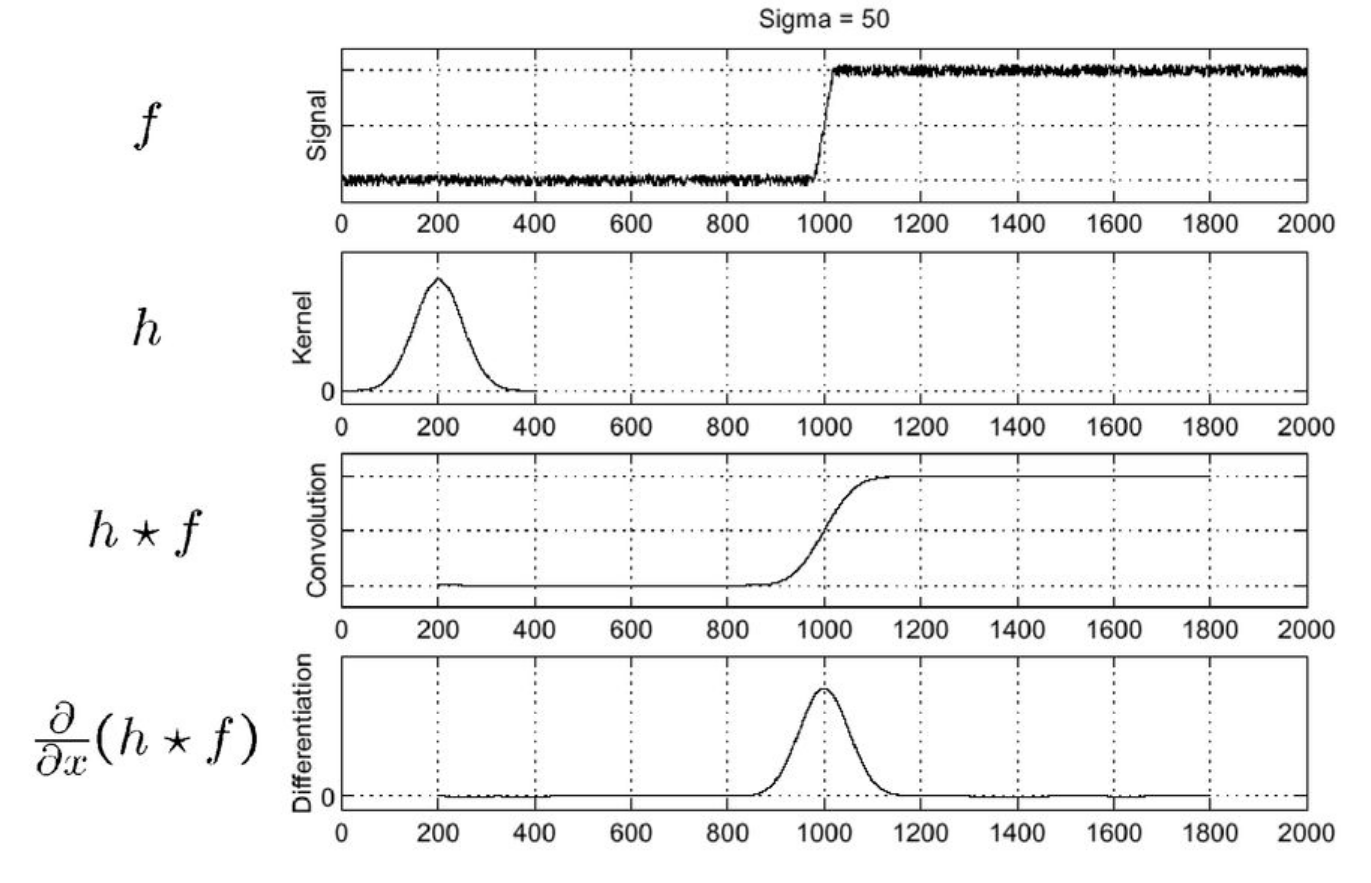
\includegraphics[scale=0.3]{figures/l3-1.png}
  \caption{\label{fig:Gaussian smoothing} Effect of Gaussian smoothing on noisy function}
\end{figure}

In order to find edges in such an example, simply look for peaks in $\frac{\delta}{\delta x}(h \star f)$, where $h\star f$ is $f$ convolved with the kernel $h$.

Convolution has many nice properties including being transitive and composable, allowing us to say that $\frac{\delta}{\delta x}(h \star f) \equiv (\frac{\delta}{\delta x}h) \star f$, this allows us to store the gaussian derivative as a filter and perform one less step when finding the edges in a noisy function $f$.

There are other popular kernels including Prewitt, Sobel and Roberts.

Every smoothing mask has the following properties:

\begin{itemize}
  \item Positive values
  \item all values sum to 1, as they take averages from surrounding pixels this makes sure the overall intensity of the image stays the same in areas of constant intensity.
  \item Amount of smoothing is proportional to the size of the mask
        \item They remove \textit{high frequency} components, meaning the filter also acts as a \textit{low-pass} filter.
\end{itemize}

We sometimes want to go further, we can take the second derivative by finding the derivative of our gaussian derivative filter, this is known as the \textbf{Laplacian of Gaussian} filter $ \nabla^{2} h_{\sigma} = \frac{\delta^{2}}{\delta x^{2}}h$. When this filter is applied the edge is where the resulting graph crosses the $x$ axis. These results are often more precise than the 1st derivative.

The size, $\sigma$ of our kernel effects the sharpness and the structures found, choosing \(\sigma\) depends on the task at hand.

\subsection{Laplacian Pyramid}

This operation can be performed recursively and works by taking an image $L_{i}$ and convolving it with our gaussian filter t produce $G_{i}$, this resulting smoothed image is then upscaled by injecting 0s in between each row and column before applying the Laplacian operator to produce an image $L_{i}$. As $i \rightarrow n$, the edges in $L_{i}$ get thicker.

As $i$ increases, only the thicker edges are present.


\section{Edge detection and matching}

We have seen the first step in edge detection in the previous section, smoothing. We will now look at the subsequent steps of \textbf{Edge enhancement} whereby we increase the contrast between edges and the background (via differentiation) and \textbf{Edge localisation} where we determine which local maxima are edges and which are noise.

\subsection{Thresholding}

The process of thresholding is as follows:

\begin{itemize}
  \item Choose a threshold $t$
  \item set any pixels less than $t$ to 0
  \item Set any pixels greater than $t$ to 1
\end{itemize}

The standard thresholding procedure can also be defined formally as:

\[
  E(x,y) = \begin{cases}
    1 & \text{if } \| \nabla f(x,y) \| > t \text{ for some threshold } t\\
    0 & \text{otherwise}
  \end{cases}
\]

This process can only select \textit{strong} edges and does not guarantee \textit{continuity}.

\subsection{Hysteresis Thresholding}

An alternative method of thresholding is known as \textbf{Hyteresis thresholding}. It uses 2 thresholds $t_{l},t_{h}$, to represent a high and low boundary.

\textbf{Note:} usually $t_{h} = 2t_{l}$.

\begin{align*}
  & \|\nabla f(x,y) \| \geq t_{h} && \text{definitely an edge} \\
  t \geq & \| \nabla f(x,y) \| < t_{h} && \text{maybe an edge, depends on the neighbouring pixel classifications} \\
  & \| \nabla f(x,y) \| < t_{l} && \text{definitely not an edge}
\end{align*}

Results of hysteresis thresholding often have better contour connectivity, i.e. more likely for entirely of edge to be preserved.

\begin{algorithm}
  \caption{Hysteresis Thresholding}
  \ForEach{position $(x,y)$}{
    \uIf{if $\|\nabla f(x,y) \| < t_{h}$}{discard pixel $(x,y)$}
    \Else{keep pixel $(x,y)$ as it is \textbf{strong}, and definitely an edge}
  }
  \ForEach{kept pixel}{
    \ForEach{connected pixel $(x,y)$ (different notions of connectedness see Section~\ref{subsec:connectedness})}{If $\| \nabla f(x,y) \| \geq t_{l}$ re-add the pixel, it is a part of an edge}
  }
\end{algorithm}

\subsection{Non-maximum supression}



This is a thinning operator, and transforms wide \textit{ridges} to a single pixel wide.

It does this by removing non-maximal pixels whilst preserving edge connectivity.

It does this by:

\begin{itemize}
  \item Checking if a pixel is a local maxima along the gradient direction
  \item Selecting a single maximum across the width of the edge

        This sometimes requires interpolation if the gradient direction points towards the middle of 2 pixels.
\end{itemize}


\label{sssec:non-max}

\begin{figure}[ht]
  \centering
  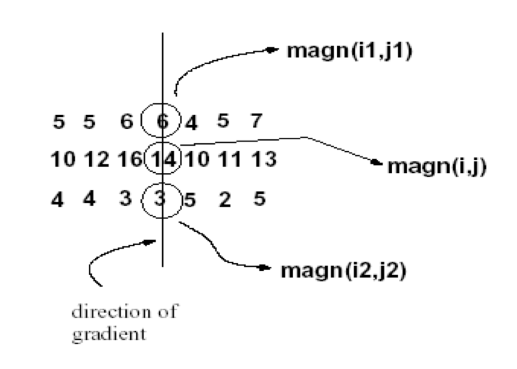
\includegraphics[scale=0.5]{figures/l3-2.png}
  \caption{\label{fig:non-max} Non-maximum suppression}
\end{figure}


\begin{algorithm}
  \caption{Non-Maximum Suppression}
  \For{each pixel $(x,y)$}{
    \uIf{$magn(i,j) < magn(i_{1},j_{1})$ or $magn(i,j) < magn(i_{2},j_{2})$}{
      $I_{N}(i,j) =0$
    }
    \Else{
      $I_{N}(i,j) = magn(i,j)$
    }
  }
\end{algorithm}
\subsection{Designing an Edge Detector}

We have the following criteria for an \textit{optimal} edge detector:

\begin{enumerate}
  \item \textbf{Good detection}

        An optimal detector will minimise the probability of false positives i.e. \textit{``edges''} caused by noise. They will also minimise false negatives, the case in which true edges are missed

  \item \textbf{Good localisation}

        Detected edges should be close to or at the same position as the true edges

  \item \textbf{Specificity}

        A detector should return only a single point per true edge, i.e. edges should be sharp and not blurred over many pixels.
\end{enumerate}

\subsection{Canny Edge Detector}

\textit{Canny came up with it, it isn't a particularly shrewd model.}

This is the most popular edge detector in computer vision.

Canny showed that the first derivative of a Gaussian well approximates the operator that optimises a trade-off between signal-to-noise ratio and localisation.

The process of the Canny edge detector is as follows:

\begin{itemize}
  \item Filter image using the derivative of Gaussian
  \item Calculate the gradient magnitude and direction
  \item Perform non-maximum suppression (See Section~\ref{sssec:non-max})
  \item Linking and thresholding using hysteresis thresholding

        We apply the high threshold to initialise contours, we then trace these contours until the magnitude falls below the low threshold.
\end{itemize}

\subsubsection{Canny Characteristics}

The Canny operator gives images with edges which are single pixel wide with good continuation between adjacent pixels. It is one of the most widely used edge detection operators and there are many sub-types. It is very sensitive to parameters, requiring extensive tuning for different domains.

\section{Binary Image Analysis}
Binary images are black and white, silhouette images.

Advantages:
\begin{itemize}
  \item They are easy to aquire/take
  \item They require low amount of space to store
  \item They are (relatively) simple to process
\end{itemize}

Disadvantages:
\begin{itemize}
  \item  They have limited utility
  \item They cannot generally capture 3D scenes
  \item Specialised equipment is required to capture silhouettes.
\end{itemize}

The basic steps of binary image analysis are as follows:

\begin{enumerate}
  \item Convert the image into a binary format\

        This can be done by thresholding
  \item Clean up the thresholded image

        This is performed using \textbf{morphological operators}
  \item Extact separate \textit{blobs}
  \item Describe the blobs with region properties
\end{enumerate}

\subsection{Converting to binary form}

We do this by thresholding, this is where we take a greyscale image and convert it to a binary mask.

We can use standard thresholding, hysteresis thresholding or a mask:

Where we have a set of values $Z$ which define the intensity values which we are interested in:

\[
  E(x,y) = \begin{cases}
    1 & \text{if } \| \nabla f(x,y) \|\in Z \\
    0 & \text{otherwise}
  \end{cases}
\]

\subsection{Morphological operators}

These are operators used to change the shape of the foreground regions via intersection/ union operations between a scanning structuring element and a binary image.

This is a useful operation to \textit{clean up} the results from thresholding.

The basic operations used are \textbf{Dilation} and \textbf{Erosion}.


\subsubsection{Dilation}

This operation expands connected components, grows features and fills in holes in the image. An example of what this operation does can be seen in Figure~\ref{fig:dilation-eg}

\begin{figure}[ht]
  \centering
  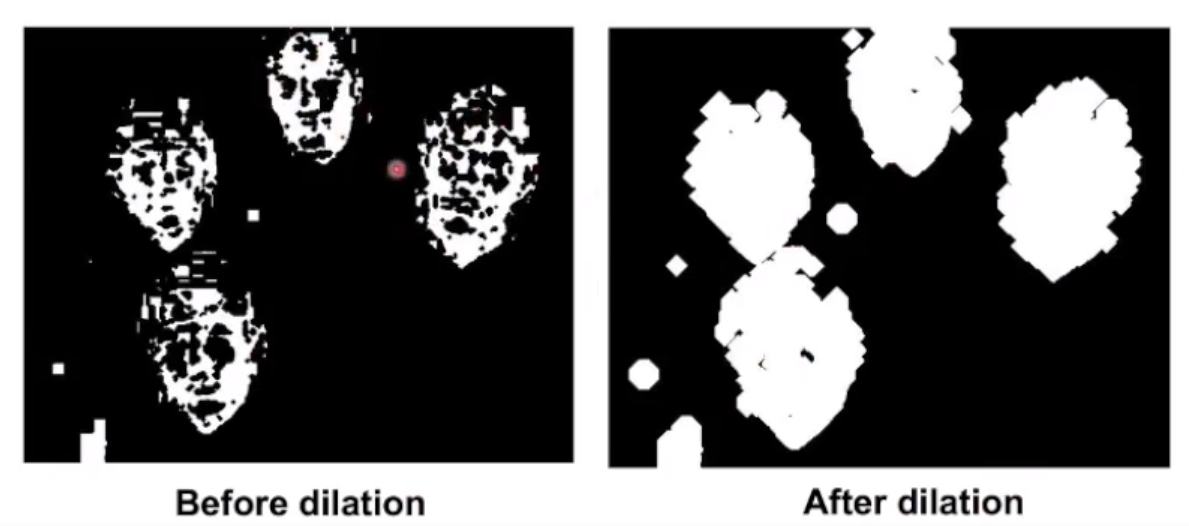
\includegraphics[scale=0.3]{figures/l3-3.png}
  \caption{\label{fig:dilation-eg} Before and after Dilation operation}
\end{figure}

At each position, if the current pixel is \textit{on}  i.e. is 1, then set all the output pixels corresponding to structuring element to 1.

This operation can be seen in a stream of binary pixels in Figure~\ref{fig:dilation-eg2}. You can see that the \textit{objects}  have become larger as gaps have been filled in. This procedure can scale to 2D images through the use of 2D mask.

\begin{figure}[ht]
  \centering
  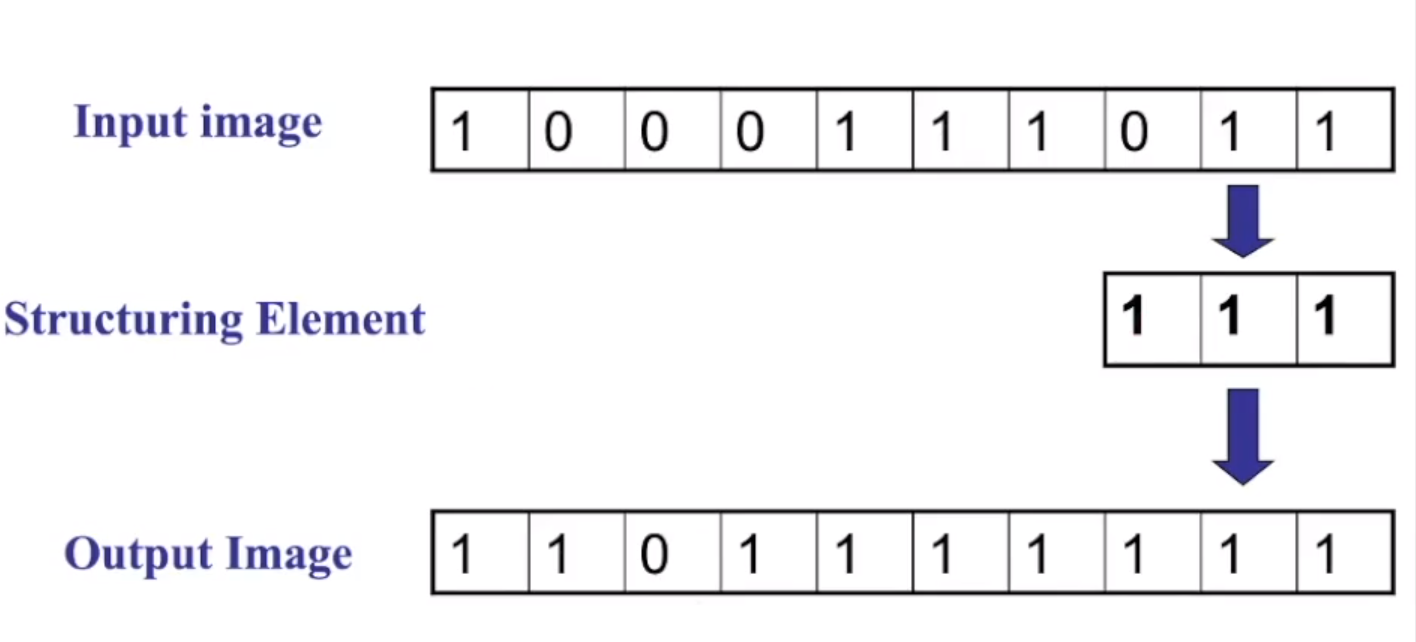
\includegraphics[scale=0.2]{figures/l3-5.png}
  \caption{\label{fig:dilation-eg2} Dilation on a stream of binary pixels}
\end{figure}



\subsubsection{Erosion}

This operation \textit{erodes}  connected components, shrinks features and removes \textit{bridges, branches}  and noise.

An example of what it does to the result of our Dilation operation can be seen in Figure~\ref{fig:erosion-eg}

\begin{figure}[ht]
  \centering
  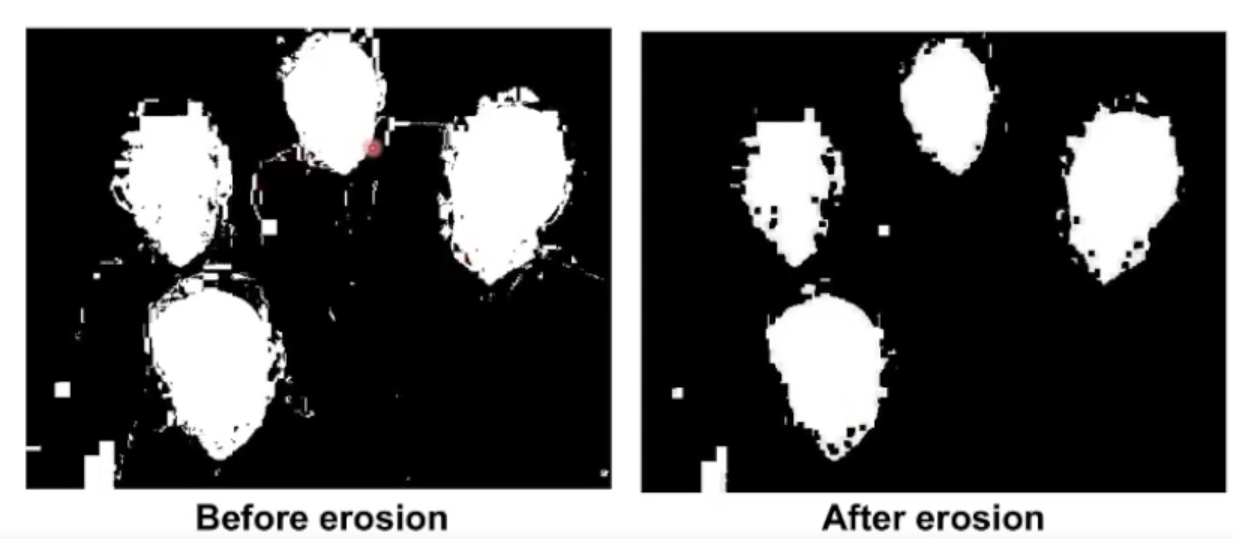
\includegraphics[scale=0.3]{figures/l3-4.png}
  \caption{\label{fig:erosion-eg} Erosion Example }
\end{figure}

To perform the erosion operation:

If every pixel under the structuring element is 1, then set the output pixel corresponding to the current pixel to 1, see Figure~\ref{fig:erosion-eg2}. Notice that the \textit{object} get smaller.

\begin{figure}[ht]
  \centering
  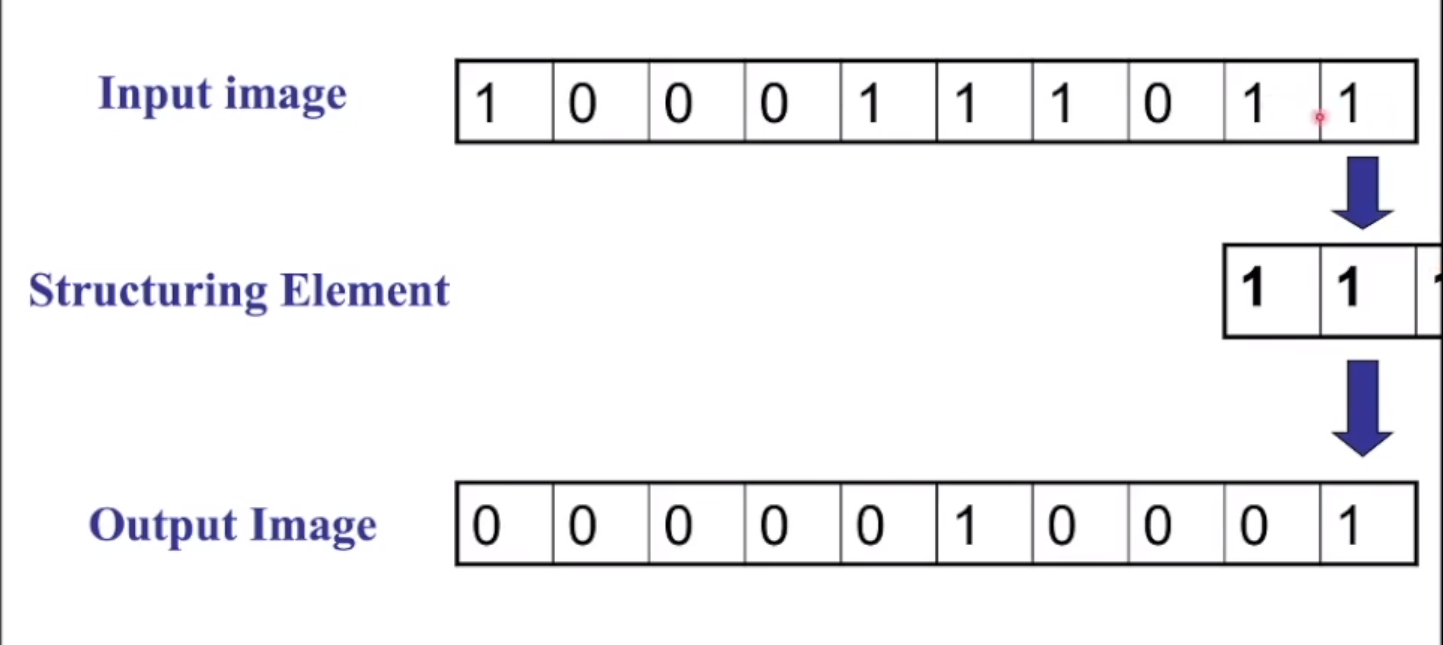
\includegraphics[scale=0.2]{figures/l3-6.png}
  \caption{\label{fig:erosion-eg2} Erosion applied to binary pixel stream}
\end{figure}

\subsection{Opening}

Opening is the process of performing erosion and then dilation to a binary image. This process removes small objects but keep the original shape.

\subsection{Closing}

Closing is the process of performing dilation followed by erosion to a binary image. This fills in holes and keeps the original shape.

\subsection{Connectedness}
\label{subsec:connectedness}

How do we determine what pixels are \textit{connected} to eachother when attempting to filter out noise without removing object detail?

Connectedness is the process of defining which pixels are considered neighbours.

\subsubsection{4-Connected}

This is the notion that a pixel is connected to others if it shares \textit{northerly, easterly, southerly} or \textit{westerly} border with them.

\subsubsection{8-Connected}

This is an extension of 4-Connectedness, here a pixel is deemed connected to all 8 of the pixels surrounding it, adding the diagonally connected pixels to the 4-Connected notion.


\subsection{Region Properties}

Given connected components, we can compute many simple \textit{features} per blob including:

\begin{itemize}
  \item Area, defined as the number of pixels in the region
  \item The centroid, the average $x$ and $y$ position of pixels in the region
  \item The bounding box, the minimum and maximum coordinates in both directions.
\end{itemize}

\end{document}
